
\chapter{Open Loop LTI Systems} \label{LA_chapter}

The transient response analysis carried out in this chapter is based on using a representation with  transfer functions of the system output according to his input. The use of this particular representation is more intuitive for the process engineer, since it consists of a simple input-output representation, where if it take into account that for its study the input has been set a priori, the transient output can predicted immediately from the analysis of the system transfer function.

\vspace{0.4cm}
To do this, consider the open loop system of the Fig. \ref{chp_la_fig01_la}.

\begin{figure}[H]
	\centering
	\includegraphics[scale=1.2]{./figuras/chapter_gla/fig_la.png}
	\caption{Open loop LTI system}
	\label{chp_la_fig01_la}
\end{figure}
where \textit{Y}(\textit{s}) = \textit{G}(\textit{s})\textit{U}(\textit{s}) with \textit{G}(\textit{s}) a polynomial ratio written as,

\begin{equation}\label{eqn01_chp_la}
	G(s)=\frac{b_m s^m \dots b_1 s + b_0}{s^n+a_1s^{n-1}+\dot a_{n-1}s^1 + a_n}
\end{equation}

Note that the dynamic response turns out to be,
\begin{equation}\label{eqn02_chp_la}
	y(t)= \mathscr{L}^{-1} \left[ \frac{b_m s^m \dots b_1 s + b_0}{s^n+a_1s^{n-1}+\dot a_{n-1}s^1 + a_n} U(s)\right]
\end{equation}
where the available inputs in this application are step and impulse.


\section{Impulse response}\index{inpulse!response}

Impulse response \index{impulse response} is the system dynamic response subjected to the input signal equal to a Dicrac delta input (denote as $\delta(t)$).

Thus, being the temporary expression of an unit impulse $u(t) = \delta(t)$, its Laplace transform results $U(s) = \mathscr{L}[u(t)] = \mathscr{L}[\delta(t)] = 1$ then,  \textit{Y}(\textit{s}) = \textit{G}(\textit{s}) and the dynamic LTI system response is,

\begin{equation} \label{Eq06_chp_trans}
y(t) = \mathscr{L}^{-1}[G(s)] ~~\mbox{.}
\end{equation}

In conclusion, \textit{the impulse response of a linear system is equal to the inverse transformation of its plant transfer function.}

\vspace{0.4cm}
\textbf{Example 1} \label{ejem01_gla_oct}

%\begin{example} \label{ejem01_gla_oct}
	Consider a linear system whose transfer function is,
	\begin{equation}\label{eqn_Gs_ejem01}
		G(s)=\frac{(s+1)}{s^2+ 0.5 s +1}
	\end{equation}
	subject to a Dirac Delta input. We pretend to obtain the dynamic system response  subject to such excitation.
	
	\vspace{0.4cm}
	To do this, before carrying out a simulation, we will make a study based on the transfer function of the system.
	
	\vspace{0.4cm}
	\begin{enumerate}
		\item \textbf{Stability:} It is possible to determine this based on the poles of the system transfer function, in this case under open loop. To do this, using Octave, you can determine these poles using the following commands:
		
		\vspace{0.4cm}
		%------------------------------------------------------------------------------------------------------
		% Cargo archivo de Octave para motrar en el ejemplo
		%\lstinputlisting[language=Octave,frame=single,firstline=6, lastline=16, caption=Código de Octave del Ejem. \ref{ejem01_gla_oct} para el calculo de las raíces de lazo cerrado.]{./m/chapter_la/ejem01_ltitool.m}
		%------------------------------------------------------------------------------------------------------
		
		\begin{verbatim}
		% System transfer function
		s=tf('s');
		Gs=(s+1)/(s^2+0.5*s+1);
		
		% Poles and Zeros
		polesGs=roots(Gs.den{1,1})
		\end{verbatim}
		
		\vspace{0.4cm}
		La respuesta en la ventana de comandos de Octave es:
		\begin{verbatim}
		polesGs =
		
		-0.25000 + 0.96825 i
		-0.25000 - 0.96825 i
		\end{verbatim}
		
		\item \textbf{Initial and Final Value:} These values can be determined by the initial (IVT) and final (FVT) values theorems.
		
		\vspace{0.4cm}
		Taking into account the following remark:
		
		\begin{remark}
			\begin{remarca}\label{rem01_chp_trans}
				The initial value ($t = 0^+$) of the impulse response of the self-regulating linear system itself with \textit{n} > \textit{m} is a finite magnitude.
			\end{remarca}
			
			\begin{demo}
				See Adam's textbook \cite{Adam2018}, among others.
			\end{demo}
		\end{remark}
	
	    Where it is denoted as \textit{n} the denominator polynomial order and \textit{m} that corresponding to the numerator.
		
		\vspace{0.4cm}
		According to IVT,
		
		\begin{eqnarray*}
			y(0^{+}) &=& \lim _{s \to \infty } sG(s)U(s)\\
			&=& \lim _{s \to \infty } s \frac{(s+1)}{\left ( s^2 + 0.5 s + 1 \right ) } 1\\
			&=& 0  ~~\mbox{.}
		\end{eqnarray*}
		
		\vspace{0.4cm}
		
		\begin{remark}
			\begin{remarca}\label{rem02_chp_trans}
				The final value ($t \to \infty$) of the impulse response of a self-regulating linear system itself with $n \ge m$ is zero.
			\end{remarca}
			
			\begin{demo}
				See Adam's textbook \cite{Adam2018}, among others.
			\end{demo}
		\end{remark}
		
		According to FVT,
		
		\begin{equation*} 
			y(\infty)= \lim _{s \to 0} s Y(s) = \lim _{s \to 0} s G(s)U(s) = \lim _{s \to 0} s \frac{(s+1)}{s^2+0.5 s+1}1=0
			~~\mbox{.}
		\end{equation*}
		
		
		\item \textbf{Impulse Response:} With the previously information it is possible to predict the system dynamic behavior. For this particular case, we can predict that the system leaves zero (through the IVT) and returns to zero (through the FVT). In addition, it will oscillate around the final value since such system has two complex conjugate roots, according to previous calculations.
		
		
		Also, using the \texttt{impulse}  Octave command you can determine the dynamic open-loop response of the system for a Dirac delta input, as indicated below.
		
		\begin{verbatim}
		% System transfer function
		s=tf('s');
		Gs=(s+1)/(s^2+0.5 s+1);
		
		% Impulse response
		impulse(Gs)
		\end{verbatim}
		obtaining the following graph:
		
		\begin{figure}[H]
			\centering
			\includegraphics[scale=0.55]{./m/chapter_la/impulseGs_ltitool.png}
			\caption{System impulse response (\ref{eqn_Gs_ejem01}).}
			\label{chp_la_fig02_impulse}
		\end{figure}
		
	\end{enumerate}
	
%\end{example}



\section{Step response}\index{step!response}

Now, consider the system dynamic response subjected to a step input signal with amplitude \textit{k}.

The step temporal expression is, \textit{u}(\textit{t}) = \textit{kH}(\textit{t}) where, \textit{H}(\textit{t}) is the Heavyside function and therefore, the Laplace transform of \textit{u}(\textit{t}) is \textit{U}(s) = \textit{k}/\textit{s}.  Consequently, the temporal response of the linear system results,

\begin{equation} \label{Eq08_chp_trans}
y(t) =  \mathscr{L}^{^-1} \left[G(s) \frac{k}{s}  \right]   ~~\mbox{.}
\end{equation}

That is to say: \ textit {the step response with amplitude \textit{k} of a linear system is equal to the inverse Laplace transform of the transfer function multiplied by \textit{k}/\textit{s}.}

\vspace{0.4cm}
\textbf{Example 2} \label{ejem02_gla_oct}

%\begin{example} \label{ejem02_gla_oct}
	Consider a linear system of the Exam. \ref{ejem01_gla_oct} whose transfer function is given by (\ref{eqn_Gs_ejem01}). Obtain the dynamic response of such system for a step input.
	
	\vspace{0.4cm}
	Firstly, it is studied
	
	\vspace{0.4cm}
	\begin{enumerate}
		\item \textbf{Stability:} This depends on the roots of the characteristic equation and is not affected by the type of input. Therefore, the system will have a stable open loop dynamic response for the step input.
		\item \textbf{Initial and Final Values:} They can be determined by IVT and FVT. 
		
		For IVT, the following remark is established below.
		
		\begin{remark}
			\begin{remarca}\label{rem03_chp_trans}
				The initial value of the step response of the self-regulating linear system itself is zero if \textit{n} > \textit{m} and nonzero if \textit{n} = \textit{m}.
			\end{remarca}
			
			\begin{demo}
				See Adam's textbook \cite{Adam2018}, among others.
			\end{demo}
		\end{remark}
		
		According to Eq. (\ref{eqn_Gs_ejem01}), it is easy to proof that,
		\begin{equation*} 
			y(0^+)= \lim _{s \to 0} s Y(s) = \lim _{s \to 0} s \ G(s)U(s) =  \lim _{s \to \infty} \cancel{s} \frac{(s+1)}{s^2+0.5s+1} \frac{k}{\cancel{s}} = 0 ~~\mbox{.}
		\end{equation*}
		
		
		For FVT, the following remark is established below.
		
		
		\begin{remark}
			\begin{remarca}\label{rem04_chp_trans}
				The final value of the step response of the self-regulating linear system itself is equal to \textit{kK}.
			\end{remarca}
			
			\begin{demo}
				See Adam's textbook \cite{Adam2018}, among others.
			\end{demo}
		\end{remark}
	
		Where it is denoted as \textit{k} the step amplitude  and \textit{K} to the static gain \index{static gain} of the open loop plant.
		
		\vspace{0.4cm}
		According to the FVT and taking into account Eq. (\ref{eqn_Gs_ejem01}) it is possible to write,
		
		\begin{equation*} 
			y(\infty)= \lim _{s \to 0} s Y(s) = \lim _{s \to 0} s \ G(s)U(s) = \lim _{s \to 0} \cancel{s} \frac{(s+1)}{s^2+0.5s+1} \frac{k}{\cancel{s}} =  k
		\end{equation*}
		
		\item \textbf{Step response:}
		With the previously determined information, the system dynamic behavior  can be predicted for the amplitude input step \textit{k}. For this example particular, it can be predicted that the system leaves zero (IVT) and reaches a final value equal to \textit{kK} (FVT). In addition, the dynamic response will oscillate around the final value since such system has two complex conjugate roots, according to  previously calculus.
		
		
		In addition, using the Octave command \texttt{step} , the dynamic open loop response of the system can be determined, as indicated below.
		
		\begin{verbatim}
		% System transfer function
		s=tf('s');
		Gs=(s+1)/(s^2+0.5*s+1);
		
		% Step response
		step(Gs)
		\end{verbatim}
		
		Thus the Fig. \ref{chp_la_fig03_step} is obtained.
		
		\begin{figure}[H]
			\centering
			\includegraphics[scale=0.55]{./m/chapter_la/stepGs_ltitool.png}
			\caption{System step response (\ref{eqn_Gs_ejem01}).}
			\label{chp_la_fig03_step}
		\end{figure}

	\end{enumerate}



%\end{example}


\section{Tool Developed for Open Loop Systems}

This tool allows:
\begin{enumerate}
	\item To determine poles and zeros maps of a transfer function.
	\item Similarly, impulse and step dynamic responses of \textit{G}(\textit{s}) are presented in the main application window. Also, it is necessary to specify,
	\begin{enumerate}
		\item step amplitude, in case of choosing for this option and
		\item simulation time.
	\end{enumerate}
\end{enumerate}

Also in this developed tool additional information is presented, as
\begin{enumerate}
	\item Stability or instability of the LTI system.
	\item Final value reached by the open loop system once the transient has finished.
	\item Approximate settling time, which is calculated based on the dominant poles of the system. Such calculus can be improved if the simulation time is extended.
\end{enumerate}

\vspace{0.4cm}
\textbf{Example 3}

It is pretend to obtain the open-loop response to the step and delta for the transfer function,
\begin{equation}
	G(s)=\frac{s+1}{s^2+0.5s+1}
\end{equation}
the application can be invoked in command mode as indicated below.

\begin{verbatim}	
	% packages are loaded.
	pkg load control signal ltitool
	
	% Clean memory and command window.
	clear all, clc
	
	% Complex variable  "s"
    s = tf("s");
    % plant
    Gol=(s+1)/(s^2+0.5*s+1);
    % simulation parameters
    k=1;        % step amplitude
    tFinal=20;  % simulation time


   % ------------------------------------------------------------------------
   % Poles-Zeros Map
   % ------------------------------------------------------------------------
   title_string='Poles and Zeros Map of G(s)';
   legend_zeros_string='Zeros of G(s)';
   legend_poles_string='Poles of G(s)';

   figure(1), 
   xpzmap(title_string,legend_zeros_string,legend_poles_string, ... 
   Gol.num{1,1},Gol.den{1,1});

   % ------------------------------------------------------------------------
   % Simulation
   % ------------------------------------------------------------------------
   % Step response
   figure(2), OLstepresponse(Gol.num{1,1},Gol.den{1,1},k,0.0,tFinal,1000);

   % Impulse response 
   figure(3), OLimpulseresponse(Gol.num{1,1},Gol.den{1,1},0.0,tFinal,1000);

   % ------------------------------------------------------------------------
   % Additional information 
   % ------------------------------------------------------------------------
   [stability,yinf,Test]=additionalinfo(Gol.num{1,1},Gol.den{1,1}, ...
                                       tFinal,1000)
\end{verbatim}

The command window reports
\begin{verbatim}
>> stability = Asympt. Stable
>> yinf =  1
>> Test =  16.060
\end{verbatim}


Notice that in the case of the step response, the command window reports that \texttt{yinf=1}while for the impulse response \texttt{yinf=0}.

\vspace{0.4cm}
\textbf{Example 4}

The same example can be solved directly by invoking the analysis and simulation window  of open-loop linear systems, simply by typing in the command window,
\begin{verbatim}
>> pkg load control signal ltitool,
>> oLWnd;
\end{verbatim}
and then Octave will present the window that it shows in Fig. \ref{chp_la_fig01_GLA}.

\begin{figure}[H]
	\centering
	\includegraphics[scale=0.5]{./figuras/chapter_gla/fig01_ejemGLA.png}
	\caption{Analysis and simulation window for LTI systems in open loop.}
	\label{chp_la_fig01_GLA}
\end{figure}

Notice that, 
\begin{itemize}
	\item The window has preloaded data that can be changed.
	\item It is possible to specify, step amplitude and simulation time.
	\item It can be obtained easily  (i) poles-zeros map, (ii) step response or, (iii) impulse response.
	\item The + button throws a graph out of the application window.
\end{itemize}

\vspace{0.4cm}
By way of example, the Fig. \ref{chp_la_fig02_GLA} shows the step response along with the additional  information about stability, reached steady state value and settling time.

\begin{figure}[H]
	\centering
	\includegraphics[scale=0.5]{./figuras/chapter_gla/fig02_ejemGLA.png}
	\caption{Open loop LTI system analysis and simulation window after pressing the step response button.}
	\label{chp_la_fig02_GLA}
\end{figure}



\section{Conclusions}

